\documentclass[conference]{IEEEtran}
\IEEEoverridecommandlockouts
% The preceding line is only needed to identify funding in the first footnote. If that is unneeded, please comment it out.
\usepackage{cite}
\usepackage{amsmath,amssymb,amsfonts}
\usepackage{algorithmic}
\usepackage{graphicx}
\usepackage{textcomp}
\usepackage{graphicx}
\graphicspath{ {./images/} }
\usepackage{xcolor}
\usepackage[utf8]{inputenc}
\usepackage{hyperref}
\def\BibTeX{{\rm B\kern-.05em{\sc i\kern-.025em b}\kern-.08em
    T\kern-.1667em\lower.7ex\hbox{E}\kern-.125emX}}
\begin{document}

\title{
Longest Common Prefix From Set Of Strings\\
}

\author{\IEEEauthorblockN{Aastha Singh}
\IEEEauthorblockA{IIT2019078}
\and
\IEEEauthorblockN{Vaibhav}
\IEEEauthorblockA{IIT2019079}
\and
\IEEEauthorblockN{Ranveer Singh}
\IEEEauthorblockA{IIT2019080}
}

\maketitle

\noindent \begin{abstract}

In this paper ,we have devised an algorithm to find the longest common Prefix from a set of strings. We have used the divide and conquer approach to solve the problem and also analysed the time and space complexity of the program.\\\\
Keyword : Prefix, longest common prefix, space complexity, time complexity.

\end{abstract}


\section{\textbf{Introduction}}
\noindent In this problem, we have to find the longest common prefix for given ‘N’ strings. \\

\noindent We know that the common prefix for any two strings will be the  consecutive common character from the start of the strings.\\

\noindent For example: Let string1 is “India” and string2 is “Indore”, so the common prefix for string1 and string 2 will be “Ind”.\\

\noindent The algorithm  is described in detail in \textbf{part II}.\\


\section{\textbf {Algorithm Description and Analysis}}

\begin{enumerate}

\item The algorithm asks for the number of strings ‘N’ as an input.\\

\item Now the algorithm asks for N strings which are now stored in an array.\\

\item Now we use the divide and conquer approach to solve this problem.
\\

\item The array of strings is divided into two parts. The same is done for the left part and then the right part. \\

\item We keep on dividing the arrays until we get a single string.
\\

\item Now we start returning the longest common prefix between the left and the right strings.
\\

\item The longest common prefix between two strings is calculated by simply comparing the strings by iterating through them.\\

\item At the end we will get the longest common prefix of the array of strings.
\\ \\

\textbf{For Example - }

Let StringArr[ ] = {“India”, “Indonesia”, “Indiana”, “Indian” , “IndianOcean”}\\

The array is first divided into 2 parts - \\


Arr1[ ] = { “India”, “Indonesia” }andArr2[ ] = {  “Indiana”    ,“Indian”,
“IndianOcean”}\\

Now Arr1[] is divided into 2 parts :-\\\\
Arr11[ ] = {“India” }\\
Arr12[ ] = { “Indonesia” }\\

Since the size is 1 ( only one string in the arrays ) these strings are returned.\\
Now for Arr1 the string returned from the left part is “India” and the string returned from the right part is “Indonesia”.\\

We calculate the longest common prefix of the two strings, which comes out to be “Ind” and return it.\\

Now similarly this happens for Arr2[ ].\\

Arr21[ ] = { “Indiana” } \\
Arr22[ ] = { “Indian”, “IndianOcean” } \\

Arr22 returns “Indian”\\\\

Now the returned “Indian” and “Indiana” are compared so “Indian” is returned.\\

Now finally the string returned from left part of StringArr is “Ind” and the string returned from the right part of StringArr is “Indian” \\

The final answer returned is longest common Prefix of “Ind” and “Indian” which is “Ind”.\\

So, we get “Ind” as the answer.\\ \\ \\


\end{enumerate}

\section{\textbf{Pseudo Code}} 
\noindent Function lcp \\
Pass In: string s[ ], int lo, int hi\\
\begin{algorithmic}
	\IF {$lo == hi$} 
		\STATE return s[hi]
	\ENDIF
	\IF {$hi > lo$}
	  \STATE  $mid \gets lo+(hi-lo)/2 $
	   \STATE	$str1 \gets lcp(s,lo,mid)$
	    \STATE	$str2 \gets lcp(s,mid+1,hi)$
        \STATE   $res  \gets  {""}$
        \STATE  $n1 \gets str1.size() $
        \STATE  $n2 \gets str2.size()$ 
        \IF  {$n1\le n2$} 
            \STATE	$sz=n1$
        \ELSE	
            \STATE	$sz=n2$
        \ENDIF
        \FOR{$i=0$,$i<sz$,i{+}{+}} 
            \IF {$str1[i]==str2[i]$} 
                \STATE $res.push(str1[i])$
             \ELSE 
                \STATE $break$
            \ENDIF
        \ENDFOR
    \ENDIF \\
return res
\end{algorithmic}

\section{\textbf {Time Complexity}}
\noindent Since in the lcp function, we are iterating through all the strings in the string array so the complexity of the function will be O(n*m) where n is the total number of strings in the array of strings and m is the length of the longest string among them.

\begin{figure}[htp]
    \centering
    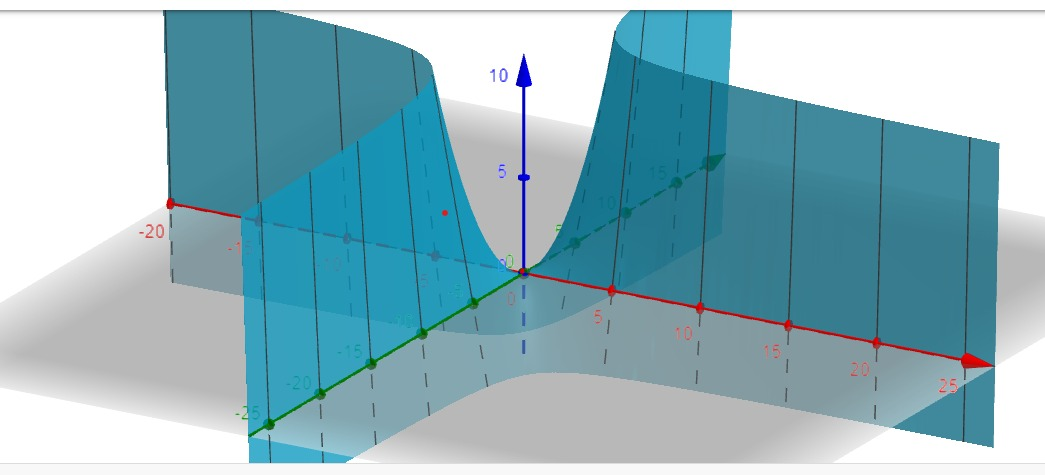
\includegraphics[width=8cm]{TimeComplexity}
    \caption{Time complexity curve}
    \label{fig:timecomplexity}
\end{figure}

\section{\textbf {Auxiliary Space Complexity}}
\noindent The auxiliary space complexity of the program is O(m*log(n)). This is because we allocate space to the resultant string or the longest common prefix string. There will be a maximum of log(n) divisions and each string returned will have a maximum size of m.

\begin{figure}[htp]
    \centering
    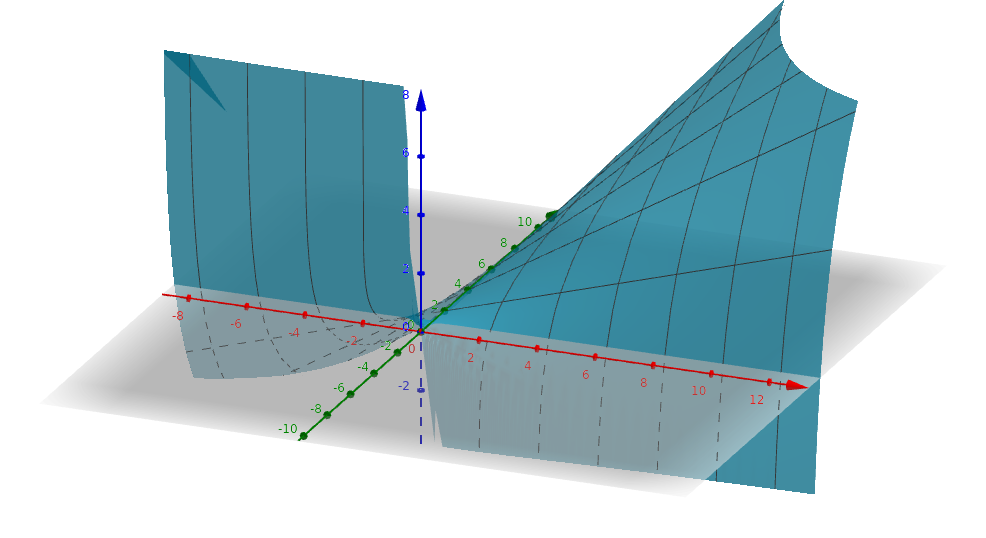
\includegraphics[width=8cm]{AuxiliarySpaceComplexity}
    \caption{Auxiliary space complexity curve}
    \label{fig:AuxiliarySpaceComplexity.png}
\end{figure}

\section{\textbf {Conclusion}} \noindent We have arrived at the solution of the problem by the divide and conquer method, where we are iterating through all the characters of all the strings, so we can say that the time complexity is O(N*M), where N = Number of strings and  M = Length of the largest string.\\

\section{\textbf {References}} 

\begin{enumerate}

\item  \href{https://edutechlearners.com/download/Introduction_to_algorithms-3rd%20Edition.pdf}{Introduction to Algorithms}\\
    
\item  \href{https://stackoverflow.com/questions/49436211/longest-common-prefix-divide-and-conquer-approach-complexity-analysis}{
Stackoverflow}
\\
\item  \href{https://www.geeksforgeeks.org/longest-common-prefix-using-divide-and-conquer-algorithm}{GeeksforGeeks}

\end{enumerate}

\end{document}
